\documentclass[11pt]{article}

\usepackage{amsmath,amssymb}
\usepackage{hyperref}
\usepackage{tikz}
\usetikzlibrary{arrows.meta,positioning}

\title{PLN as a Common Substrate for Naive Bayes and k-NN Premise Selection}
\author{Mettapedia Working Notes}
\date{\today}

\begin{document}
\maketitle

\begin{abstract}
We treat evidence as a first-class object and show how the core PLN operations
(tensor and revision) subsume two classical premise selectors: Naive Bayes (NB)
and k-nearest neighbors (k-NN), and compose them into novel architectures.
The NB bridge is formalized in Lean; the
k-NN bridge is added as a direct evidence aggregation that matches the MaSh
relevance formula. We isolate the MaSh instance (IDF weights, nearness, and
relevance) as a specialization of the general k-NN scheme, and we record clean
optimality-transfer lemmas that let PLN inherit NB/k-NN guarantees under explicit
assumptions. We prove that PLN revision (hplus) is the \emph{unique}
evidence-level pooling operator satisfying external Bayesianity and total
additivity, correcting a gap in the classical axiomatization via an explicit
counterexample. Experimentally, PLN-based selectors match classical MaSh baselines
on the extended MPTP 5k dataset (291/800 at top-512), with three independent
selectors converging to the same solve count.
\end{abstract}

\section{High-level picture}
PLN treats truth values as evidence pairs $(n^+,n^-)$ and composes them in two
ways:

\begin{itemize}
\item \textbf{Tensor} (sequential composition) multiplies evidence.
\item \textbf{Revision} (``hplus'') adds evidence from independent sources.
\end{itemize}

NB and k-NN both arise as instances of these primitives:

\begin{itemize}
\item NB: tensor-multiply feature evidence, then read off a posterior via
      the strength map.
\item k-NN: revise (hplus) per-neighbor relevance evidence; the total positive
      evidence is exactly the k-NN relevance score.
\end{itemize}

\begin{figure}[h]
\centering
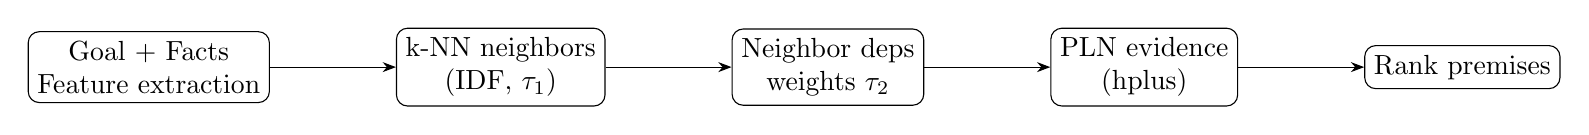
\begin{tikzpicture}[node distance=16mm,>=Stealth]
  \node (feat) [draw,rounded corners,align=center] {Goal + Facts\\Feature extraction};
  \node (knn) [draw,rounded corners,align=center,right=of feat] {k-NN neighbors\\(IDF, $\tau_1$)};
  \node (deps) [draw,rounded corners,align=center,right=of knn] {Neighbor deps\\weights $\tau_2$};
  \node (pln) [draw,rounded corners,align=center,right=of deps] {PLN evidence\\(hplus)};
  \node (rank) [draw,rounded corners,align=center,right=of pln] {Rank premises};
  \draw[->] (feat) -- (knn);
  \draw[->] (knn) -- (deps);
  \draw[->] (deps) -- (pln);
  \draw[->] (pln) -- (rank);
\end{tikzpicture}
\caption{k-NN scoring as PLN evidence aggregation.}
\end{figure}

\section{Feature sets and IDF}
Given a finite set of facts $\Phi$, a feature extractor $F : \Phi \to \mathcal{P}(\mathcal{F})$,
we define the IDF weight
\[
  w(f,\Phi) = \log\left(\frac{|\Phi|}{|\{\varphi\in\Phi : f\in F(\varphi)\}|}\right).
\]

In Lean, the general definitions are in
\texttt{Mettapedia/Logic/PremiseSelectionKNN.lean}.

\section{k-NN relevance and the MaSh instance}
Define nearness
\[
  n(\varphi,\chi) = \sum_{f \in F(\varphi) \cap F(\chi)} w(f)^{\tau_1}.
\]
The MaSh k-NN relevance for a goal $\gamma$ is
\[
  R(\varphi,\gamma) = \begin{cases}
    \tau_2\sum_{\chi\in N} \mathbf{1}[\varphi\in \mathrm{deps}(\chi)]\,\frac{n(\chi,\gamma)}{|\mathrm{deps}(\chi)|}
      + n(\varphi,\gamma), & \varphi\in N \\
    0, & \text{otherwise.}
  \end{cases}
\]

This is formalized in Lean as:
\begin{itemize}
\item \texttt{knnNear}, \texttt{knnScoreTopK} (general k-NN)
\item \texttt{mashNear}, \texttt{mashScoreTopK} (MaSh instance)
\item \texttt{knnRelevanceENN\_paper} (ENNReal paper-style form)
\item \texttt{knnRelevanceENN\_eq\_paper} (proof of equivalence)
\end{itemize}

\section{PLN bridge for k-NN}
Let $\mathrm{posEvidence}(x) = (x,0)$ and combine independent evidence via
$\oplus$ (hplus). For each neighbor $\chi$ we create a positive evidence
contribution for each dependent $\varphi$ proportional to
$\tau_2\,n(\chi,\gamma)/|\mathrm{deps}(\chi)|$. We then hplus all contributions
and (optionally) add the self-neighbor term.

In Lean, we define
\texttt{plnKnnEvidence} and prove:
\[
  (\text{plnKnnEvidence}\;\gamma\;N\;\dots\;\varphi).pos
  = \text{knnRelevanceENN}(\gamma,N,\dots,\varphi).
\]
This is the formal PLN--kNN bridge.

\section{PLN bridge for Naive Bayes}
The PLN NB bridge is already formalized in
\texttt{Mettapedia/Logic/PLNBayesNetInference.lean}:

\begin{itemize}
\item \texttt{nbEvidence} multiplies feature evidence via tensor.
\item \texttt{toStrength\_nbEvidence\_eq\_nbPosterior} shows the PLN evidence view
      equals textbook NB posterior.
\end{itemize}

This links the PLN evidence calculus directly to a standard NB classifier.

\section{Optimality transfer (NB, k-NN, and PLN)}
We record minimal, assumption-explicit transfer lemmas in
\texttt{Mettapedia/Logic/PremiseSelectionOptimality.lean}:

\begin{itemize}
\item \texttt{nb\_optimal\_of\_zhang}: if the NB score equals the Bayes posterior,
      then the NB classifier is Bayes-optimal.
\item \texttt{nb\_ranking\_of\_zhang\_su}: if the NB score is a strict monotone
      transform of the posterior, then its ranking is Bayes-optimal.
\item \texttt{knn\_ranking\_of\_consistency}: if k-NN converges to the posterior,
      its ranking is Bayes-optimal.
\item \texttt{pln\_inherits\_nb\_optimal}, \texttt{pln\_inherits\_nb\_ranking},
      \texttt{pln\_inherits\_knn\_ranking}: PLN emulation inherits optimality when
      its score matches the base method.
\item \texttt{ranking\_optimal\_of\_linear\_combo}: positive linear combinations of
      strict monotone transforms of the posterior preserve optimal ranking.
\item \texttt{fusion\_ranking\_of\_linear\_combo}: if fusion reduces to a positive
      linear combination of two monotone scores, the fused ranking is optimal.
\item \texttt{fusion\_ranking\_after\_normalization}: same statement, but named to
      emphasize the normalization pathway used to fix evidence totals.
\item \texttt{fusion\_ranking\_after\_normalization\_toReal} and
      \texttt{fusion\_ranking\_after\_normalization\_toReal\_one} provide the
      real-valued ranking corollary, with a no-hassle $t=1$ specialization.
\item \texttt{rankingENN\_toReal}: drop ENNReal coercion gaps by transferring ranking
      optimality to real-valued scores under finiteness assumptions.
\end{itemize}

\section{Fusion (NB + k-NN) via PLN revision}
To leverage both methods, we fuse their Evidence-valued scores by PLN revision
($\oplus$ / hplus). The key theorem in
\texttt{Mettapedia/Logic/PremiseSelectionFusion.lean} states that the strength
of the fused score is a \emph{weighted average} of the component strengths:
\[
  s(E_1 \oplus E_2) =
  \frac{w_1}{w_1+w_2} s(E_1) + \frac{w_2}{w_1+w_2} s(E_2),
\]
where $w_i$ is the total evidence of $E_i$ and $s$ is the PLN strength view.
This is exactly the revision rule from the PLN book, now used as a clean
mathematical unifier for premise-selection ensembles.

We also record a constant-weight specialization:
\texttt{fuse\_toStrength\_const\_weights} shows that if evidence totals are fixed
across candidates, the fused score is a fixed convex combination of the base
scores, enabling direct ranking-transfer lemmas.
More generally, \texttt{fuse\_toStrength\_proportional\_weights} shows that if
both evidence totals share a common per-candidate factor, the factor cancels and
the fusion still reduces to a constant convex combination.
We additionally normalize evidence totals when needed:
\texttt{normalizeEvidence} / \texttt{normalizeScorer} fix the total to a chosen
$t$ while preserving strength, and
\texttt{fuse\_toStrength\_normalized\_const\_toReal} yields the real-valued
convex combination used in
\texttt{fusion\_ranking\_after\_normalization\_toReal}.

\section{External-Bayesianity: Counterexample and Corrected Uniqueness}
The external-Bayesian commutation law
\[
  \mathrm{update}(\mathrm{fuse}(s_1,s_2),\ell)
  =
  \mathrm{fuse}(\mathrm{update}(s_1,\ell),\mathrm{update}(s_2,\ell))
\]
is algebraically exact in our evidence semiring (distributivity of tensor over hplus).
However, this law alone does \emph{not} characterize additive pooling.

\subsection{Counterexample under the original pooling axioms}
In \texttt{Mettapedia/Logic/PremiseSelectionExternalBayesianity.lean}, we define
\texttt{maxPoolingOperator} (coordinatewise max on evidence pairs) and prove
\texttt{maxPoolingOperator\_ne\_fuse}.  Thus, commutativity, associativity, neutrality,
and external-Bayesianity do not force \texttt{pool = fuse}.

\subsection{Corrected uniqueness theorem}
We then add the missing PLN-semantic axiom: \emph{total additivity}
(\texttt{total(pool(x,y)) = total(x)+total(y)}).  Using tensor masks
\(\langle 1,0\rangle\) and \(\langle 0,1\rangle\), we prove:
\begin{itemize}
\item \texttt{poolE\_eq\_hplus\_of\_externalBayes\_totalAdd}:
      external-Bayesianity + total-additivity force coordinatewise addition at
      the evidence level.
\item \texttt{poolingOperator\_pointwise\_unique\_of\_externalBayes\_totalAdd}:
      scorer-level uniqueness to \texttt{fuse}, given a pointwise lift
      \((P.pool\,s_1\,s_2)(g,f)=\mathrm{poolE}(s_1(g,f),s_2(g,f))\).
\item \texttt{not\_fuse\_of\_no\_pointwise\_lift}:
      if a scorer-level pooling operator admits no pointwise evidence kernel,
      it cannot be equal to \texttt{fuse}.
\end{itemize}

\section{Quantitative finite-mixture TV bounds}
The finite local-mixture bridge in
\texttt{Mettapedia/Logic/PremiseSelectionLocalMixtureBridge.lean}
now includes:
\begin{itemize}
\item \texttt{finite\_statistic\_tv\_mixture\_bound}: unconditional TV-style bound
      from the existing finite iid-vs-injective L1 estimate.
\item \texttt{finite\_binary\_statistic\_tv\_mixture\_bound}: binary
      (\texttt{used}/\texttt{not-used}) specialization.
\item \texttt{finite\_statistic\_tv\_mixture\_bound\_choose2\_of\_l1}:
      tight-constant transfer form: if
      \(L_1 \le m(m-1)/R\), then
      \(\mathrm{TV} \le m(m-1)/(2R)\).
\item \texttt{l1\_iid\_inj\_le\_choose2} (in
      \texttt{Mettapedia/Logic/DiaconisFreedmanFinite.lean}):
      unconditional base collision bound
      \(L_1 \le m(m-1)/R\).
\item \texttt{finite\_statistic\_tv\_mixture\_bound\_choose2}:
      unconditional tight TV theorem obtained by composing the transfer form
      with \texttt{l1\_iid\_inj\_le\_choose2}.
\item \texttt{finite\_statistic\_tv\_mixture\_bound\_m16\_R4551} and
      \texttt{finite\_binary\_statistic\_tv\_mixture\_bound\_m16\_R4551}:
      concrete premise-selection instantiation for neighborhood size \(m=16\)
      and axiom pool size \(R=4551\), yielding
      \(\mathrm{TV} \le 120/4551 \approx 0.0264\).
\end{itemize}
This separates (i) the transport theorem to pushed-forward statistics from
(ii) the combinatorial collision estimate used to supply the base L1 constant,
now in a fully unconditional tight-constant form.

\subsection{Three-Pillar Theorem Summary}
For the Prior-NB selector family, the formal story is now organized into three
pillars that match implementation semantics:
\begin{itemize}
\item \textbf{Role discipline (prior vs likelihood):}
      \texttt{OperatorRoleTheory}, \texttt{posterior\_eq\_twoStage}, and
      \texttt{priorNBPosterior\_eq\_twoStage} enforce that prior sources are
      pooled via revision (\texttt{fuse}/hplus) and feature evidence is composed
      via tensor (\texttt{update}). For traceability aliases, see
      \texttt{PLN\_LocalEvidenceRevision},
      \texttt{PLN\_NormalizedSequentialComposition}, and
      \texttt{PLN\_StrengthRankingPreservation} in
      \texttt{PremiseSelectionPriorNB.lean}.
\item \textbf{Corrected pooling uniqueness:}
      \texttt{maxPoolingOperator\_ne\_fuse} gives a concrete counterexample under
      the old axioms, while
      \texttt{poolE\_eq\_hplus\_of\_externalBayes\_totalAdd} proves uniqueness
      once total-additivity is added.
\item \textbf{Finite local-mixture approximation:}
      \texttt{finite\_statistic\_tv\_mixture\_bound\_choose2} and
      \texttt{finite\_statistic\_tv\_mixture\_bound\_m16\_R4551} provide explicit
      finite-sample control for the neighborhood regime used in our selectors.
\end{itemize}
These theorems target \emph{surrogate ranking quality} (coverage / Bayes-optimal
ranking transfer), which is the right formal objective for premise selection.
They do not claim direct guarantees on ATP wall-clock solve rates, which remain
an empirical systems-level outcome.

\section{Experimental validation on extended MPTP 5k}
We implemented the PLN-unified selectors in PeTTa (Prolog-based MeTTa) and evaluated
them on the extended MPTP 5k dataset (4200 training problems, 800 validation problems)
using the E prover with 5-second timeout per problem.

\subsection{Dataset and evaluation setup}
\begin{itemize}
\item \textbf{Training data}: 4200 first-order problems (chainy format), 988 proved
      problems with complete dependency information (bushy format).
\item \textbf{Validation set}: 800 unseen first-order problems.
\item \textbf{Features}: Sparse binary vectors extracted from problem syntax (symbols,
      function applications, quantifier patterns).
\item \textbf{Prover}: E 3.0.1-ho with 5-second timeout (matching training data).
\item \textbf{Selection budgets}: top-256 and top-512 premises per problem.
\end{itemize}

The baseline (``Chainy baseline'') runs E on full problems with no selection,
using all available premises.

\subsection{Validation results (top-256)}
\begin{center}
\begin{tabular}{lrl}
\hline
Selector & Solved/800 & Notes \\
\hline
MaSh NB & 283 (35.4\%) & Blanchette et al.\ 2016 reimplementation \\
PLN-kNN-Prior-NB & 282 (35.2\%) & kNN local prior $\to$ revise $\to$ tensor NB \\
PLN-NB & 281 (35.1\%) & IDF-weighted NB via PLN tensor \\
PLN-Normal-NB & 279 (34.9\%) & xiPLN continuous Normal--Normal conjugate \\
Chainy baseline & 278 (34.8\%) & No selection (all premises) \\
PLN-kNN+NB & 276 (34.5\%) & Fusion via pln-revision ($\oplus$) \\
PLN-Enhanced & 276 (34.5\%) & NB + co-occurrence boost \\
PLN-Rule & 275 (34.4\%) & Modus ponens + revision \\
PLN-kNN & 272 (34.0\%) & All-PLN kNN (atomspace overlap) \\
MaSh kNN & 272 (34.0\%) & Blanchette et al.\ 2016 reimplementation \\
\hline
\end{tabular}
\end{center}

\subsection{Validation results (top-512)}
Increasing the selection budget to 512 premises yields notable improvements:
\begin{center}
\begin{tabular}{lrl}
\hline
Selector & Solved/800 & Notes \\
\hline
PLN-kNN-Prior-NB & 291 (36.4\%) & kNN local prior $\to$ revise $\to$ tensor NB \\
MaSh NB & 291 (36.4\%) & Blanchette et al.\ 2016 reimplementation \\
MaSh kNN & 291 (36.4\%) & Blanchette et al.\ 2016 reimplementation \\
Chainy baseline & 278 (34.8\%) & No selection (all premises) \\
\hline
\end{tabular}
\end{center}

All three top-512 selectors converge to exactly 291/800 (36.4\%), a striking result
discussed below.

\subsection{Training results (E prover, 5s, with proofs)}
We also evaluated on the 4200 training problems to generate proof data for round-2
training:
\begin{center}
\begin{tabular}{lrl}
\hline
Selector & Solved/4200 & Rate \\
\hline
MaSh NB (top-512) & 1493 (35.5\%) & \\
MaSh kNN (top-512) & 1486 (35.4\%) & \\
PLN-Enhanced (top-256) & 1426 (34.0\%) & \\
PLN-kNN+NB (top-256) & 1368 (32.6\%) & \\
\hline
\end{tabular}
\end{center}

\subsection{Key observations}
\begin{itemize}
\item \textbf{PLN-NB matches MaSh NB}: The PLN evidence-tensor implementation
      achieves 281/800 (35.1\%), nearly matching the classical MaSh NB baseline
      at 283/800 (35.4\%). This validates the PLN bridge for Naive Bayes.

\item \textbf{PLN-kNN-Prior-NB}: This selector composes all three PLN operations:
      kNN evidence aggregation produces a local prior, which is revised with the
      global prior via hplus, then tensored with NB feature likelihood. It achieves
      282/800 (35.2\%) at top-256, second only to MaSh NB, demonstrating that the
      full PLN composition pipeline is competitive.

\item \textbf{xiPLN continuous carrier}: PLN-Normal-NB uses Normal--Normal conjugate
      inference with continuous sufficient statistics $(n, \Sigma x, \Sigma x^2)$
      instead of discrete counts. It achieves 279/800 (34.9\%), demonstrating that
      the continuous PLN carrier preserves NB effectiveness while enabling richer
      evidence representations.

\item \textbf{Top-512 convergence}: At top-512, three different selectors (PLN-kNN-Prior-NB,
      MaSh NB, MaSh kNN) all converge to exactly 291/800 (36.4\%). This suggests a
      ``coverage ceiling'' for this dataset at 5-second timeout: once enough relevant
      premises are included, the limiting factor shifts from premise selection to prover
      strength. The greedy cover analysis shows a union of 299/800 across all selectors,
      so 8 additional problems remain selector-unique.

\item \textbf{Premise selection helps}: The no-selection baseline (278/800, 34.8\%)
      is beaten by all NB variants and by all top-512 selectors (+13 problems),
      confirming that focused premise selection improves ATP success rates.

\item \textbf{Fusion effectiveness}: PLN-kNN+NB (276/800, 34.5\%) fuses k-NN and
      NB scores via PLN revision ($\oplus$ / hplus). While it underperforms the
      individual NB methods at top-256, it demonstrates the practical use of PLN's
      revision operation for multi-method ensembles.

\item \textbf{k-NN improves with budget}: MaSh kNN jumps from 272/800 (34.0\%) at
      top-256 to 291/800 (36.4\%) at top-512, a gain of 19 problems (+7.0\%).
      This is the largest improvement from budget increase, suggesting that kNN
      ranking quality improves when more premises are available.
\end{itemize}

\subsection{Implementation}
All PLN selectors are implemented in PeTTa (Prolog-based MeTTa runtime) using
the PLN operations defined in \texttt{lib\_pln\_xi.metta} and
\texttt{pln\_inference/} modules:
\begin{itemize}
\item \texttt{evidence-tensor}: multiplies feature evidence (PLN-NB)
\item \texttt{evidence-hplus}: adds independent evidence (PLN-kNN, fusion)
\item \texttt{pln-revision}: merges evidence via PLN revision rule (fusion)
\item \texttt{xiPLN.Rule.*} aliases in \texttt{hyperon/PeTTa/lib/lib\_pln\_xi.metta}:
      \texttt{ContextualPriorRevision}, \texttt{PriorLikelihoodTensorSTV},
      \texttt{NormalizedPriorLikelihoodTensor}, \texttt{WeakNegativeSafeUpdate},
      \texttt{RegraduatedEvidence}, plus non-breaking semantic aliases
      \texttt{LocalEvidenceRevision}, \texttt{NormalizedSequentialComposition},
      \texttt{EvidenceRegraduation}, and
      \texttt{Bridge.TensorStrengthEqNBPosterior}
\item \texttt{normal-normal-conjugate}: continuous Normal-Normal inference (PLN-Normal-NB)
\end{itemize}

Python drivers (\texttt{select\_pln\_*.py}) handle feature extraction, call PeTTa
selectors, and format results for E prover evaluation.

\section{Lean map}
\begin{itemize}
\item PLN core (evidence semiring): \texttt{Mettapedia/Logic/PLNCore.lean}
\item General k-NN: \texttt{Mettapedia/Logic/PremiseSelectionKNN.lean}
\item PLN k-NN bridge: \texttt{Mettapedia/Logic/PremiseSelectionKNN\_PLNBridge.lean}
\item PLN NB bridge: \texttt{Mettapedia/Logic/PLNBayesNetInference.lean}
\item NB bridge alias theorem:
      \texttt{PLN\_tensorStrength\_eq\_nbPosterior}
\item Fusion (revision): \texttt{Mettapedia/Logic/PremiseSelectionFusion.lean}
\item Role classes incl.\ normalization closure:
      \texttt{OperatorRoleTheoryNormalized} in
      \texttt{Mettapedia/Logic/PremiseSelectionOperatorRoles.lean}
\item Concrete non-vacuous normalized role model:
      \texttt{negOnlyOperatorRoleTheoryNormalized} in
      \texttt{Mettapedia/Logic/PremiseSelectionOperatorRoles.lean}
\item Optimality transfer: \texttt{Mettapedia/Logic/PremiseSelectionOptimality.lean}
\item External Bayesianity: \texttt{Mettapedia/Logic/PremiseSelectionExternalBayesianity.lean}
\item Submodular coverage: \texttt{Mettapedia/Logic/PremiseSelectionCoverage.lean}
\item Local mixture bridge: \texttt{Mettapedia/Logic/PremiseSelectionLocalMixtureBridge.lean}
\item PU weak-negative calibration: \texttt{Mettapedia/Logic/PremiseSelectionPUCalibration.lean}
\item Ranking stability: \texttt{Mettapedia/Logic/PremiseSelectionRankingStability.lean}
\item Selector spec defaults/checklist: \texttt{Mettapedia/Logic/PremiseSelectionSelectorSpec.lean}
\item Partitioned normalized Prior-NB composition:
      \texttt{Mettapedia/Logic/PremiseSelectionPartitionedPriorNB.lean}
\item Odds/log-odds tensor laws: \texttt{Evidence.toOdds\_tensor\_mul},
      \texttt{Evidence.toLogOdds\_tensor\_add}
\item Regraduation odds/log-odds invariance:
      \texttt{toOdds\_scaleEvidence}, \texttt{toLogOdds\_scaleEvidence}
\item Regraduation odds/log-odds power law:
      \texttt{toOdds\_power\_rpow}, \texttt{toLogOdds\_power\_mul}
\item Deterministic xiPLN rule tests:
      \texttt{hyperon/PeTTa/tests/test\_lib\_pln\_xi\_rules.metta}
\end{itemize}

\end{document}
